\section{\normalsize Уравнение Ван-дер-Ваальса как модель неидеального газа. Изотермы газа Ван-дер-Ваальса. Критические параметры. Приведённое уравнение Ван-дер-Ваальса, закон соответственных состояний.}
\paragraph{Уравнение Ван-дер-Ваальса.}
$$\left(P+\dfrac{a\nu^2}{V^2}\right)\left(V-\nu b\right)=RT$$
Выведем его, основываясь на $PV=\nu RT$:\\
\begin{minipage}{100mm}
	Во-первых, учтем размеры молекул: \\$\dfrac{4}{3}\pi(2r)^3=8\cdot\dfrac{4}{3}\pi r^3$ --- недоступный объем для второй частицы $\Rightarrow$ в расчете на 1 молекулу $$\dfrac{1}{2}(8\cdot\dfrac{4}{3}\pi r^3)=4V_0$$
	где $V_0=4\pi r^3/3$ --- объем одной молекулы. 
\end{minipage}
\begin{minipage}{5mm}
	\quad
\end{minipage}
\begin{minipage}{65mm}
	\begin{figure}[H]
		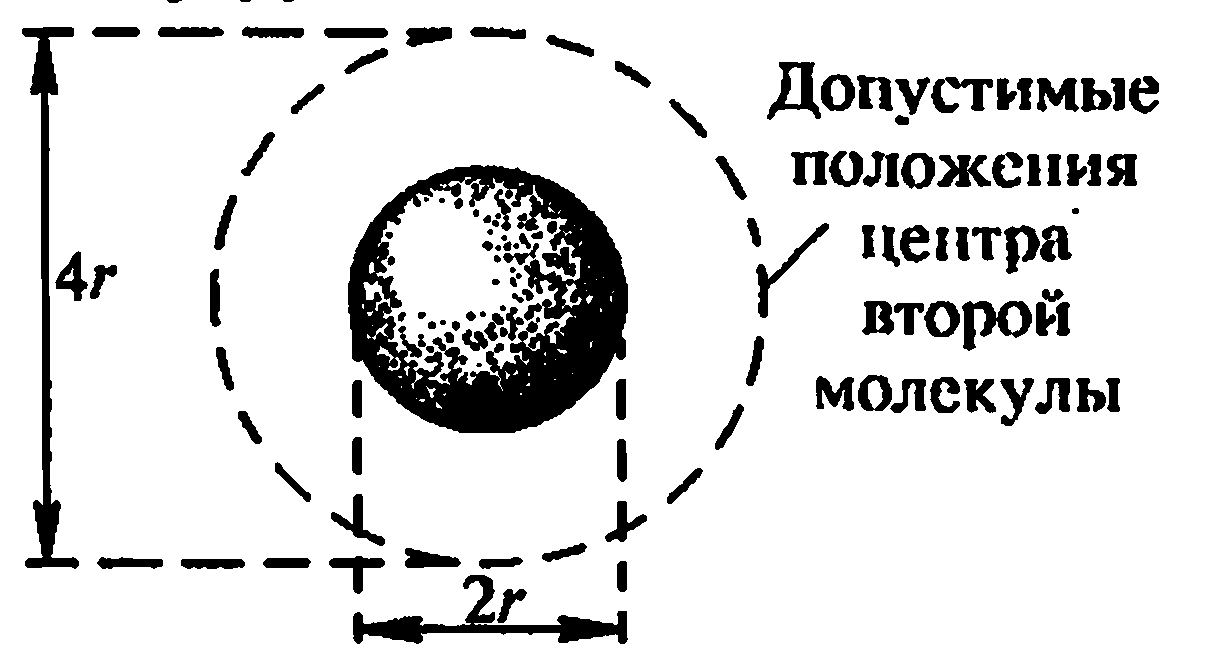
\includegraphics[width=65mm]{ris19.png}
		\caption{Учет конечности размеров молекул}
	\end{figure}
\end{minipage}

В результате объем, разрещенный для движения молекул, cоставит
$$V_\text{доп.} =V-\nu b,\quad$$
$$ b\simeq4\cdot\text{(объем молекулы в одном моле)}=4N_AV_0$$
Во-вторых, учтем, что молекулы притягиваются другк другу. Одним из механизмотв 
\begin{minipage}{65mm}
	\begin{figure}[H]
		\label{dipol}
		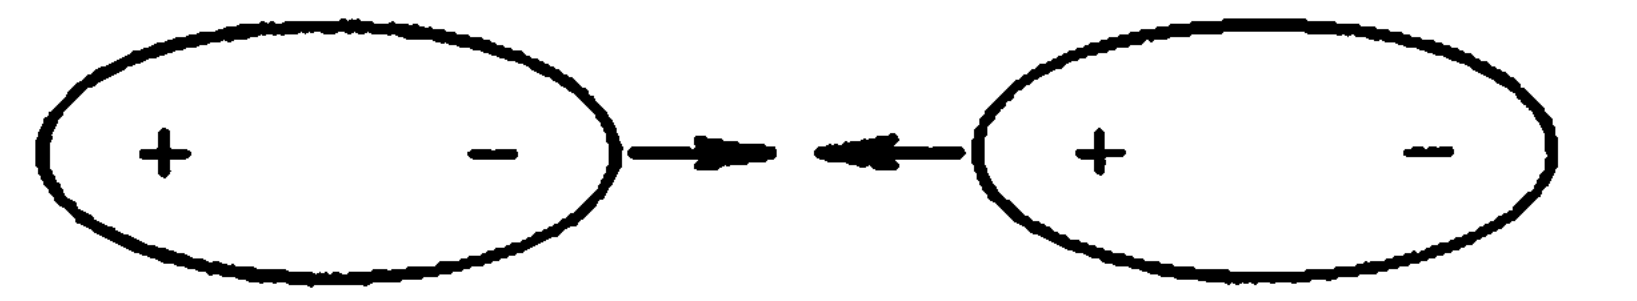
\includegraphics[width=65mm]{ris19_2.png}
		\caption{Молекулы--диполи \\притягиваются друг к другу}
	\end{figure}
\end{minipage}
\begin{minipage}{5mm}
	\quad
\end{minipage}
\begin{minipage}{100mm}
	такого притяжения может быть перераспределение зарядов и образование диполей (см. рис 2).\\
	Давление газа определяется столкновениями молекул со стенкой. Сила, действующая на молекулу у стенки со стороны газа $\sim n$, где $n$ --- число частиц. Частота соударений $\sim n$, значит давление уменьша-
\end{minipage}\\[1mm]
ется на $\Delta P\sim n^2$. Переходя от плотности $n$ к объему $V$ по формуле $n=\dfrac{\nu N_A}{V}$, мы можем записать поправку к давлению в виде $\Delta P=a_1n^2=a(\nu/V)^2.$ Окончательно это даёт
$$\left(P+\dfrac{a\nu^2}{V^2}\right)\left(V-\nu b\right)=RT$$
Величины $a$ и $b$ называется параметрами Ван-дер-Ваадбся. Параметре $a$ учитывает притяжение, а $b$ --- отталкивание молекул.
\paragraph{Изотермы газа Ван-дер-Ваальса.}